%
% Frontmatter - Introducción. Los miembros del tribunal que juzgan los PFC's tienen muchas más memorias que leer, por lo que
%	agradecerán cualquier detalle que permita facilitarles la vida. En este sentido, realizar una pequeña introducción,
%	comentar la organización y estructura de la memoria y resumir brevemente cada capítulo puede ser una buena práctica
%	que permita al lector centrarse fácilmente en la parte que más le interesa.
%

\chapter[Introducción]{Introducción}

Neste capítulo de introdución intentarase explicar os aspectos necesarios para entender en que consiste o proxecto, o que me fixo levalo a cabo e, por último, unha explicación da estrutura da presente memoria. 

\section{Internacionalización e Localización de Software}
A internacionalización é o proceso de adaptación dun software para que este poida ser adaptado a varios idiomas e ser usado en diferentes rexións sen modificar a súa enxeñería. A localización de software consiste na adaptación de dito software a unha rexión determinada. Isto aínda que afecta fundamentalmente o idioma, tamén ten outros elementos como as divisas a forma de formatear as datas ou simbolos que nunhas areas teñen un significado e noutras outro.

Trátase dun aspecto moi importante do mundo do software pois se ven unha persoa que seipa inglés, o idioma orixe da maior parte dos programas, a internacionalización dos programas é un probelma de comodidade, para o que non entenda a lingua de Shakespeare, trátase dun problema de usabilidade. Unha persoa que non sexa nativa dixital e que non entenda inglés terá serios problemas para entender calquera software moderno non localizado.

\section{O Proxecto GNOME}
GNOME é ambiente de escritorio, unha infraestructura de desarrollo e unha comunidade de software libre.

Como ambiente de escritorio foi creado polos mexicanos Miguel de Icaza e Federico Mena en 1997 como alternativa a KDE compatible coa licencias GPL\footnote{En aquel momento KDE empregaba unha licencia QPL que aínda que era libre non era compatible GPL.}. Tratase de crear un solución software para todo o mundo poñendo interés en aspectos como a accesibilidade, a internacionalización ou a usabilidade.

Como infraestructura de desarrollo GNOME provee unha gran cantidade de aplicativos e bibliotecas para crear o programas tanto para a plataforma GNOME como para outras plataformas.

\begin{figure}[h!]
    \centering
    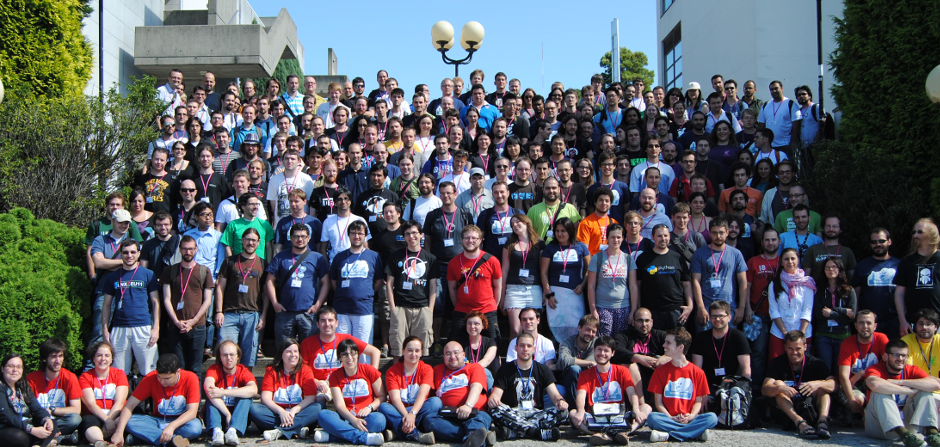
\includegraphics[width=\textwidth]{img/guadec_2012.png}
    \caption{GUADEC A Coruña 2012}
    \label{fig:guadec2012}
\end{figure}

Como comunidade reune a gran cantidade de persoas tanto voluntarias como profesionais axudaron e axudan a que o proxecto siga adiante. A comunidade GNOME en Europa reunese nas GUADEC, que é o acronimos de \textbf{G}NOME \textbf{U}sers \textbf{A}nd \textbf{D}evelopers \textbf{C}onference. No ano 2012 este encontro tivo lugar na cidade da Coruña.

\subsection{Localización e Internacionalización no Proxecto GNOME}
Como xa dixemos un dos aspectos máis importante para o proxecto GNOME é o acercamento as persoas e para lograr isto ponse pleno interés na internacionalización e na localización do ambiente de escritorio e das aplicacións de GNOME. GNOME está traducido a máis de 50 idiomas dos cales TODO teñen máis do 90\% das cadeas traducidas.

O proxecto GNOME emprega o sistema GNU Gettext para internacionalizar e localizar os seus programas e conta con unha plataforma web de nome Damned Lies para xestionar a localización de todo o proxecto. Este programa amosa as estatisticas do estado actual das traducións e axuda a xestionar o ciclo de traballo dos traductores. Permite asignar modulos a traductores, que os traductores suban os fichiros descargados e que se faga unha revisión do traballo do traductor.

Outros proxectos de software como Facebook, Twitter ou, dentro do software libre, Ubuntu contan con plataformas online dende as que se pode facer directamente a tradución. GNOME opta por facer a tradución \emph{offline} para que esta sexa dunha maior calidade.

Para que os traductores poidan traballar de forma comoda é necesario a existencia de ferramentas que lle faciliten o traballo. Estas ferramentas coñecense como CAT, que é o acronimo de Computer Assisted Translation. Neste traballo pretende realizarse unha destas ferramentas centrada no proxecto GNOME.

\section{Motivación}
Durante a GUADEC-es 2012 que tivo lugar en A Coruña dentro da GUADEC (internacional) do mesmo ano, asistín a unha charla impartida por Daniel Mustieles, o coordinador do equipo de traductores ao castelán do proxecto GNOME. Nesta charla Daniel, resaltaba a necesidade de que o programa actual de asistencia a tradución fose mellorado. GTranslator está escrito en C e emprega unha biblioteca chamada GObject para facer orientación a obxectos dentro de C. Isto fai que achegarse o proxecto sexa complicado para un novato polo que falando con outros desarrolladores da plafarma decidiuse que era mellor reescribir o programa noutra linguaxe e ao mesmo tempo arreglar alguns erros que tiña anteriormente o programa. Durante o ano seguinte presentei un proxecto para o Google Summer of Code para escribir un novo programa CAT para a plataforma GNOME. Este programa sería unha re-escritura e re-deseño de GTranaltor nunha linguaxe de programación moito máis amigable, Vala.

\section{Estrutura da memoria}

In a dolor sed odio eleifend varius. Nam ullamcorper. Curabitur ut erat vulputate nisi molestie tempus. Sed aliquam rutrum odio. In mollis. Fusce consectetuer lorem nec diam. Sed mollis lacinia purus. Curabitur feugiat hendrerit neque. Quisque auctor laoreet diam. Curabitur sit amet nisi. Fusce velit massa, dignissim quis, bibendum eget, vehicula mattis, leo. Morbi auctor leo sit amet nibh. Lorem ipsum dolor sit amet, consectetuer adipiscing elit. Nullam enim. Pellentesque hendrerit, augue non vulputate semper, sem lorem pharetra nibh, sit amet egestas massa diam ac augue. In dui nulla, egestas nec, pulvinar suscipit, tincidunt ornare, nisi. Duis tristique tortor quis magna. Vestibulum faucibus lorem nec neque. Sed nec nibh. Nunc condimentum. Maecenas neque. Nullam pretium est non risus. Etiam gravida. Maecenas nisl. Fusce pharetra odio in tortor. Integer orci turpis, interdum eget, vulputate sed, tristique a, metus. Duis vitae dui quis lectus pretium aliquam. Praesent quam.

Aliquam sed orci. Cras adipiscing nisl quis pede. Ut rhoncus. Donec viverra laoreet purus. Phasellus nulla. Vivamus eget eros. In mollis aliquam orci. Proin ullamcorper. Nullam sollicitudin vestibulum lorem. Nunc malesuada sagittis augue. Donec tellus velit, dapibus a, aliquam ac, tincidunt id, lectus.


\paragraph*{Capítulo 1.}
Phasellus tempor velit nec velit. Proin vitae dui a sapien commodo blandit. Etiam aliquam, sapien vitae fringilla venenatis, lectus sem accumsan orci, eget blandit orci odio et magna. Quisque malesuada, eros vel tempus eleifend, velit enim porttitor sem, eget consequat nulla neque et sapien. Morbi leo. Sed vestibulum lacus. Fusce ut lacus. Phasellus pellentesque pede eu eros. Duis turpis felis, eleifend ut, semper ac, porta nec, sem. Praesent odio. Sed laoreet mollis purus. Praesent vestibulum, velit ut mollis aliquam, quam lectus varius urna, sed ultricies erat nisl ac tortor. Vivamus tempor mauris sit amet nulla. Integer venenatis. Integer sagittis euismod ante. Suspendisse at elit. Duis eget purus nec pede adipiscing auctor. Proin ac est.

\paragraph*{Capítulo 2.}
Proin condimentum. Maecenas sodales. In ornare nunc a leo. Nam sit amet ligula. Nunc quis urna ac metus imperdiet lobortis. Sed quis ligula. Maecenas blandit pede. Donec lacinia rutrum ligula. Vivamus in metus vel elit pharetra molestie.

\paragraph*{Capítulo 3.}
Nullam ante lorem, placerat et, egestas nec, pellentesque non, sapien. Donec semper, felis id posuere faucibus, nibh ipsum tincidunt quam, et varius ipsum odio ac neque. In tincidunt dignissim diam. Sed lacus lorem, ornare ut, eleifend vel, pellentesque tempus, augue. Duis eu magna. Mauris libero ante, porttitor vel, lobortis a, mollis ac, sem. Nunc at lectus. Integer ac libero a nisl dignissim mollis. Donec velit neque, vestibulum eget, pulvinar vel, malesuada ut, nisi. Praesent congue tempus quam. Cum sociis natoque penatibus et magnis dis parturient montes, nascetur ridiculus mus.

\paragraph*{Capítulo 4.}
Mauris ut odio. Nulla accumsan. Morbi condimentum fermentum purus. Pellentesque habitant morbi tristique senectus et netus et malesuada fames ac turpis egestas. Nunc dignissim, neque eget convallis pretium, diam tortor fringilla lacus, a laoreet nisl metus eu magna. Cras ut lectus. Etiam accumsan feugiat elit.

\paragraph*{Capítulo ...}
Donec a pede. Proin dolor. Ut nunc ligula, tempor id, ornare sit amet, aliquam et, nibh. In mollis iaculis pede. Vivamus gravida orci eu nisl. Sed nibh sem, consequat at, iaculis non, placerat in, ligula. Praesent id nisi. Nunc pellentesque justo non libero. Sed quis est sit amet purus lobortis blandit. Sed arcu justo, rhoncus condimentum, ullamcorper iaculis, viverra et, nisl.

\paragraph*{Capítulo N.}
Fusce luctus gravida leo. Nullam dignissim arcu ac risus hendrerit rhoncus. Aliquam erat volutpat. Ut mollis, mauris non aliquam luctus, nulla sem aliquam tellus, in consequat augue odio in urna.




